% Created 2016-10-16 dom 13:47
\documentclass[11pt]{article}
\usepackage[utf8]{inputenc}
\usepackage[T1]{fontenc}
\usepackage{fixltx2e}
\usepackage{graphicx}
\usepackage{longtable}
\usepackage{float}
\usepackage{wrapfig}
\usepackage{rotating}
\usepackage[normalem]{ulem}
\usepackage{amsmath}
\usepackage{textcomp}
\usepackage{marvosym}
\usepackage{wasysym}
\usepackage{amssymb}
\usepackage{hyperref}
\tolerance=1000
\usepackage{minted}
\usepackage[spanish]{babel}
\usepackage[T1]{fontenc}
\usepackage{amsmath}
\usepackage[left=2.5cm,top=2cm,right=2.5cm,bottom=2.5cm]{geometry}
\usemintedstyle{manni}
\setminted{linenos=true}
\usepackage{graphicx}
\setcounter{secnumdepth}{0}
\author{Javier Sáez Maldonado y Luis Antonio Ortega Andrés}
\date{\today}
\title{Práctica 1 Estructura de datos.}
\hypersetup{
  pdfkeywords={},
  pdfsubject={},
  pdfcreator={Emacs 24.5.1 (Org mode 8.2.10)}}
\begin{document}

\maketitle
\section*{Ejercicio 1.}
\label{sec-1}

Teniendo el siguiente algoritmo:

\begin{minted}[]{c++}
void ordenar(int * v , int n) {

  for (int i=0; i<n-1; i++)

    for (int j=0; j<n-i-1; j++)

      if (v[j]>v[j+1]) {

	int aux = v[j]; v[j] = v[j+1]; v[j+1] = aux; } }
\end{minted}


Vamos a calcular primero su eficiencia teórica. Para ello
estableceremos según la notación O grande el peso de cada una de las
partes.

\begin{minted}[]{c++}
void ordenar(int * v, int n) {

  for (int i=0; i<n-1; i++) // (n-1)O(1) = O(n-1)

    for (int j=0; j<n-i-1; j++)// (n-1)O(1) = O(n-1)

      if (v[j]>v[j+1]) { //O(1)

	int aux = v[j]; //O(1) v[j] = v[j+1]; //O(1) v[j+1] = aux;
	//O(1)

      } }
\end{minted}

Así, como en los bucles anidados, usamos la regla del producto
O(f(n))O(g(n)) = O(f(n)g(n)) y de esta forma tenemos que "el polinomio
de la eficiencia teórica del algoritmo es" O((n-1)4*(n-1)). El 4 está
porque dentro del segundo bucle tenemos 4 operaciones que son O(1).

Sin embargo, por la notación O grande, podemos obviar los coeficientes
del monomio de mayor grado e incluso obviar los demás monomios, por lo
que el polinomio queda reducido a ser O(n$^{\text{2}}$), siendo esta la
eficiencia teórica del código.

Ahora, creamos un fichero \textbf{\textbf{ordenación.cpp}} insertando este código
para ordenar un vector. Para ello, nos hemos ayudado de los que venían
de prueba.

\begin{minted}[]{c++}
#include <iostream> include <ctime> // Recursos para medir tiempos
#include <cstdlib> // Para generación de números pseudoaleatorios

using namespace std;

void ordenar(int * v, int n) {

  for (int i=0; i<n-1; i++)

    for (int j=0; j<n-i-1; j++)

      if (v[j]>v[j+1]) {

	int aux = v[j]; v[j] = v[j+1]; v[j+1] = aux;

      } }


void sintaxis() { cerr << "Sintaxis:" << endl; cerr << " TAM: Tamaño
del vector (>0)" << endl; cerr << " VMAX: Valor máximo (>0)" << endl;
cerr << "Se genera un vector de tamaño TAM con elementos aleatorios en
[0,VMAX[" << endl; exit(EXIT_FAILURE); }


int main (int argc, char* argv[]) {

  if (argc!=3) sintaxis(); int tam=atoi(argv[1]); // Tamaño del vector
    int vmax=atoi(argv[2]); // Valor máximo if (tam<=0 || vmax<=0)
    sintaxis();

  // Generación del vector aleatorio int * v=new int[tam]; // Reserva
  de memoria srand(time(0)); // Inicialización del generador de
  números pseudoaleatorios for (int i=0; i<tam; i++) // Recorrer
  vector v[i] = rand() % vmax; // Generar aleatorio [0,vmax[

  clock_t tini; // Anotamos el tiempo de inicio tini=clock();

  ordenar(v,tam); // de esta forma forzamos el peor caso

  clock_t tfin; // Anotamos el tiempo de finalización tfin=clock();

  // Mostramos resultados cout << tam << "\t" <<
  (tfin-tini)/(double)CLOCKS_PER_SEC << endl;

  delete [] v; // Liberamos memoria dinámica

}
\end{minted}

Ahora, creamos el script que nos sirve para realizar de forma
automática las ejecuciones de nuestro programa.

\begin{minted}[]{sh}
#!/bin/csh @ inicio = 100 @ fin = 30000 @ incremento = 500 set
ejecutable = burbuja set salida = tiempos_burbuja.dat @ i = $inicio
echo > $salida while ( $i <= $fin ) echo Ejecución tam = $i echo
`./{$ejecutable} $i 10000` >> $salida @ i += $incremento end
\end{minted}

Por último, pintamos la gráfica con GNUPLOT quedando el siguiente
resultado.


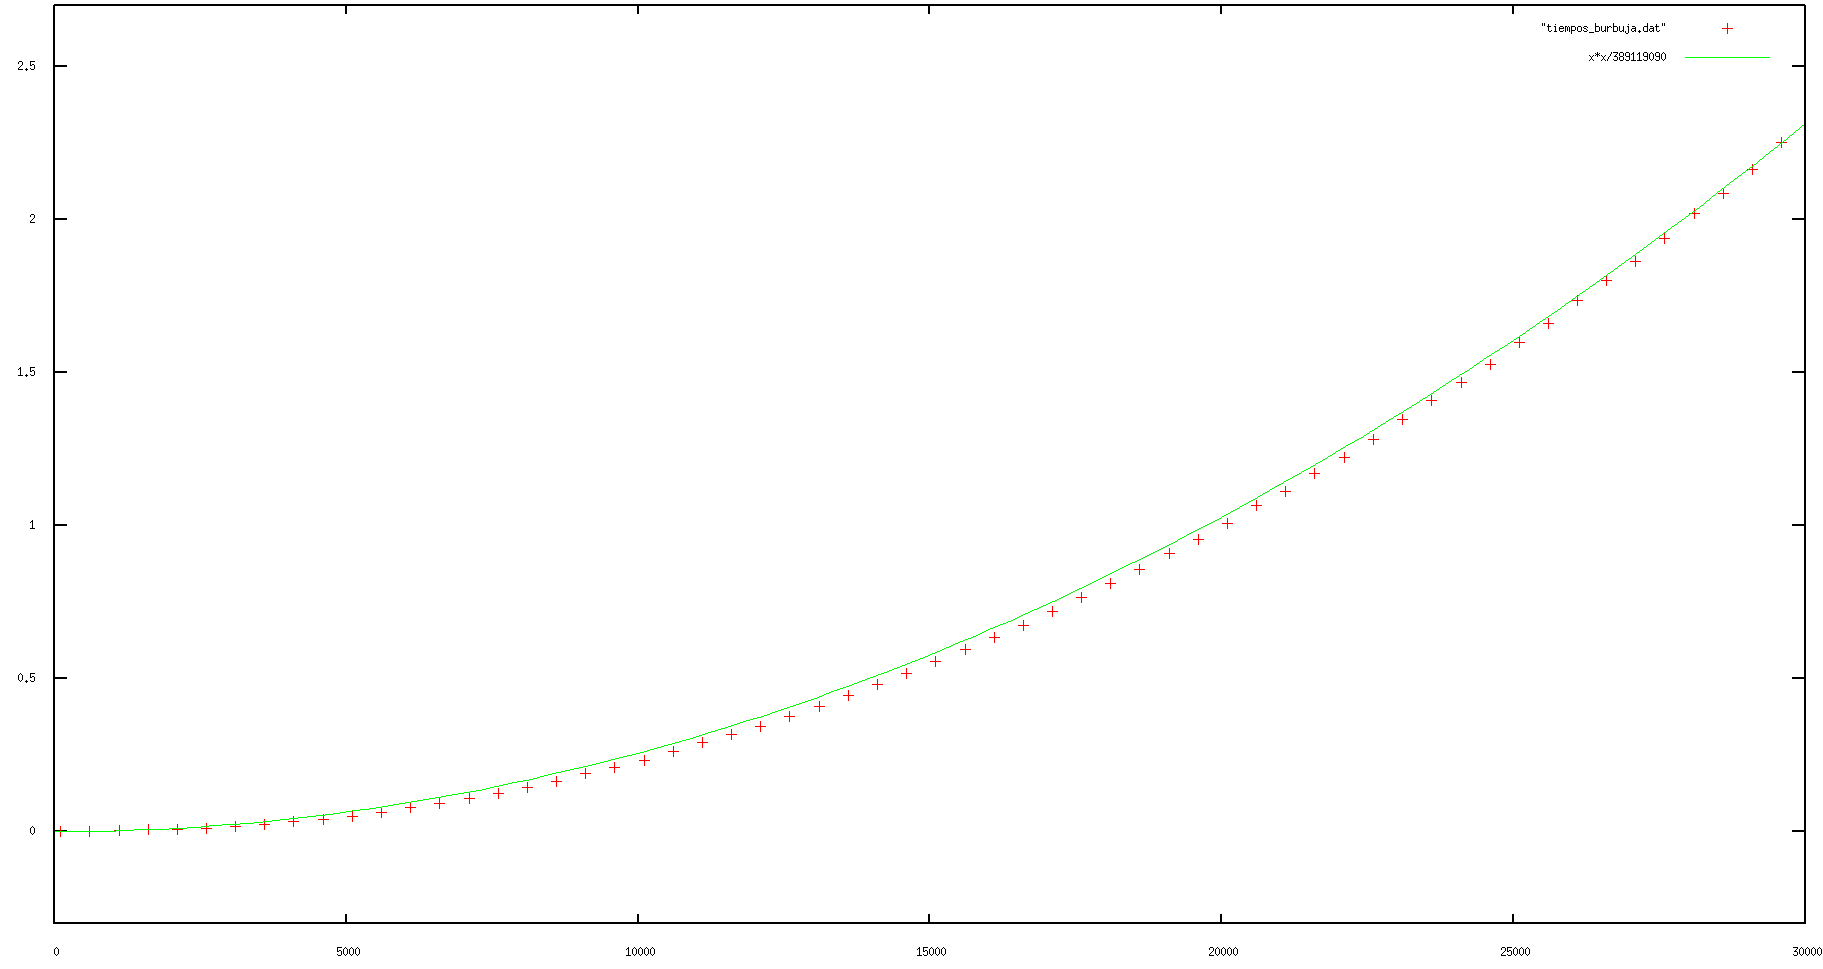
\includegraphics[scale=0.25]{grafica1.png}

Donde podemos ver que la linea verde es la eficiencia teórica y las
cruces rojas es la eficiencia resultante al ejecutar nuestro programa
en un ordenador que realiza 389119090 operaciones por segundo
ejecutando este programa.

Ya que el numero de datos no es excesivamente elevado, la eficiencia
teórica y la práctica son bastante parecidas.


\section*{Ejercicio 2.}
\label{sec-2}

Ahora, ajustamos los datos a una función cuadrática. Para ello, dentro
de GNUPLOT usamos

\begin{minted}[]{gnuplot}
f(x) = a*x**2 + b*x + c fit f(x) "tiempos_burbuja.dat" via a, b, c
plot f(x), "tiempos_burbuja.dat"
\end{minted}

Y obtenemos así esta gráfica:


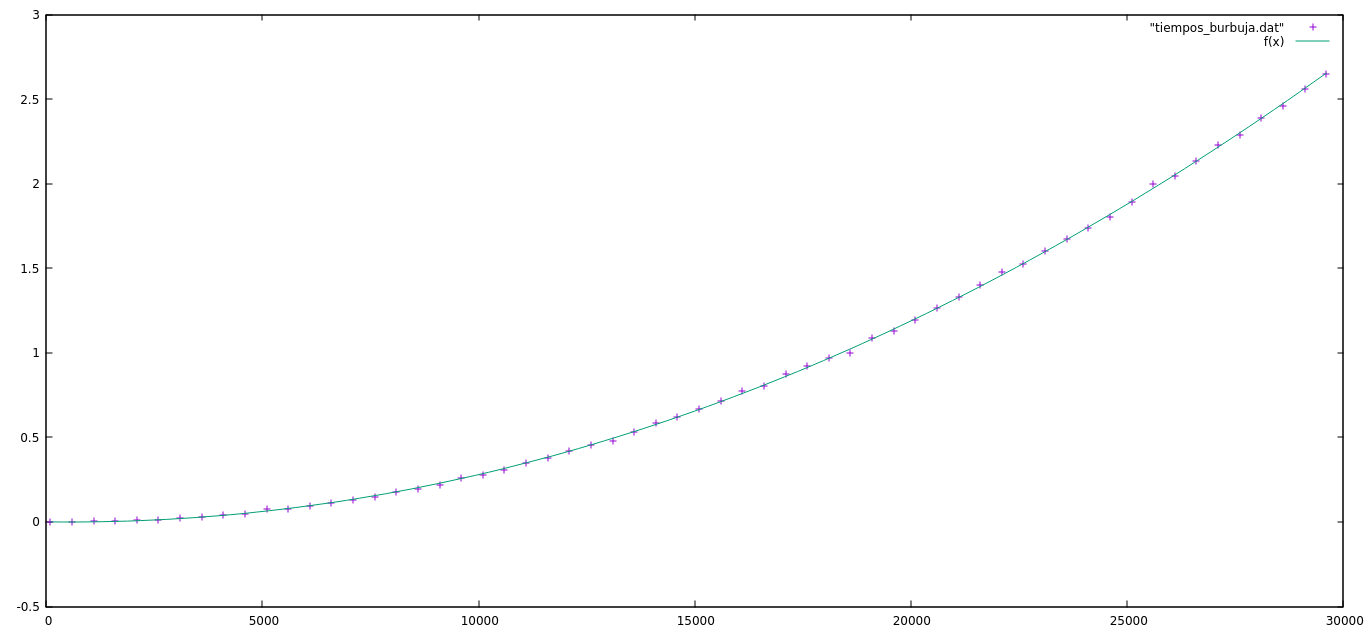
\includegraphics[scale=0.5]{Grafica2.png}


\section*{Ejercicio 3.}
\label{sec-3}

El código del ejercicio es el que hemos usado para hacer los dos
primeros ejercicios salvo la función que se realiza sobre el
vector. En este caso la función es:

\begin{minted}[]{c++}
int operacion(int * v, int n, int x, int inf, int sup) { int med;
  //Declaro una medida bool enc=false;

  while ((inf<sup) && (!enc)) { med = (inf+sup)/2; if (v[med]==x) enc
    = true; else if (v[med] < x) inf = med+1; else sup = med-1; } if
    (enc) return med; else return -1; }
\end{minted}

Lo que hace esta función (y por tanto este programa, pues se centra en
la función) es buscar un elemento en un vector, de forma que se va
primero al medio del vector y comprueba si es el elemento que
buscamos. Si no lo es, se mira si el dato buscado es es mayor, va a
volver a buscar en el mismo vector pero tomando solo la parte que
queda a la derecha de la mitad y si es menor busca en la parte que
está a la izquierda de la mitad. Para seguir buscando, vuelve a
realizar el mismo proceso que acaba de hacer en el subvector que
corresponda(de la izquierda o de la derecha).Este algoritmo es
conocido como \textbf{\textbf{búsqueda binaria}}

Calculemos ahora su eficiencia.

\begin{minted}[]{c++}
int operacion(int * v, int n, int x, int inf, int sup) { int med;
  //Declaro una medida

  bool enc=false; // O(1)

  while ((inf<sup) && (!enc)) { // O(logaritmo en base 2 de n) med =
    (inf+sup)/2; // O(1) if (v[med]==x) // O(1) enc = true; // O(1)
    else if (v[med] < x) // O(1) inf = med+1; // O(1) else sup =
    med-1; //O(1) } if (enc) // O(1) return med;// O(1) else //O(1)
    return -1; // O(1) }
\end{minted}

Primero tenemos una declaración y una declaración y asignación:
3*O(1).  Ahora, podemos ver que como tenemos un bucle usamos la \textbf{regla
del producto} y tenemos que multiplicar O($log_2 (n)$) por lo que haya
dentro del bucle, que en este caso es O(1) en la asignación y como
tenemos un \textbf{\textbf{IF/ELSE}} aplicamos la regla del máximo de ellos, que en
este caso es en todas 2*O(1) luego es irrelevante.  Después, volvemos
a tener un IF/ELSE en el que los dos son 2*O(1) y por ello la regla
del maximo tambien escoge a cualquiera de los dos.

Ahora, como todo ese código no está dentro de ningún bucle, aplicamos
la \textbf{regla de la suma} y tenemos por tanto O(3) + O($log_2 (n)$) *
O(2) + O(2) = O(3 + 2 * ($log_2 (n)$) + 2).

Sin embargo, por la notación O grande podemos resumir en que eso es
igual a O($log_2(n)$) y esta es nuestra eficiencia teórica.

Al realizar la eficiencia empírica, lo primero que hemos notado ha
sido que el programa que se nos proporciona no genera los vectores
ordenados, para solucionarlo, hemos incluido la biblioteca \emph{algorithm}
y hemos usado la función sort.  Otro problema que hemos encontrado es
que el reloj que estamos utilizando no tiene la suficiente precisión
como para ver mejor la diferencia en una escala tan baja. Para
solucionarlo, hemos cambiado el reloj a uno de la librería \emph{chrono},
que tiene fama de ser el mas preciso y hemos procedido a hacer pruebas
con esta nueva medición.  El resultado ha sido el siguiente:

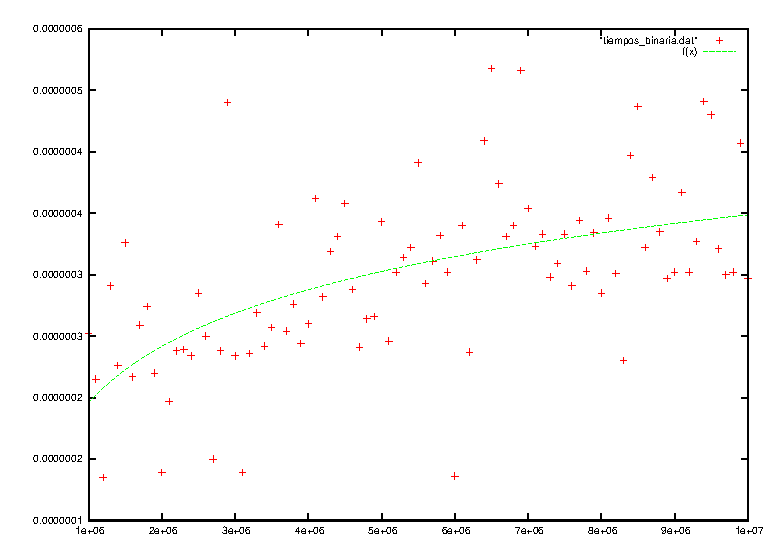
\includegraphics[scale=1]{grafica_binaria_otro.eps}

\section*{Ejercicio 4}
\label{sec-4}

Para realizar la ordenación vamos a realizar la siguiente función de
la biblioteca \emph{algorithm}:

\begin{minted}[]{c++}
sort(vector,vector+tamanio); // Para ordenar el vector de menor a
mayor.  sort(vector,vector+tamanio,greater<int>()); // Para ordenar el
vector de mayor a menor.
\end{minted}

Ahora, representamos las dos gráficas que han quedado al realizar con
un script las ejecuciones de los programas.


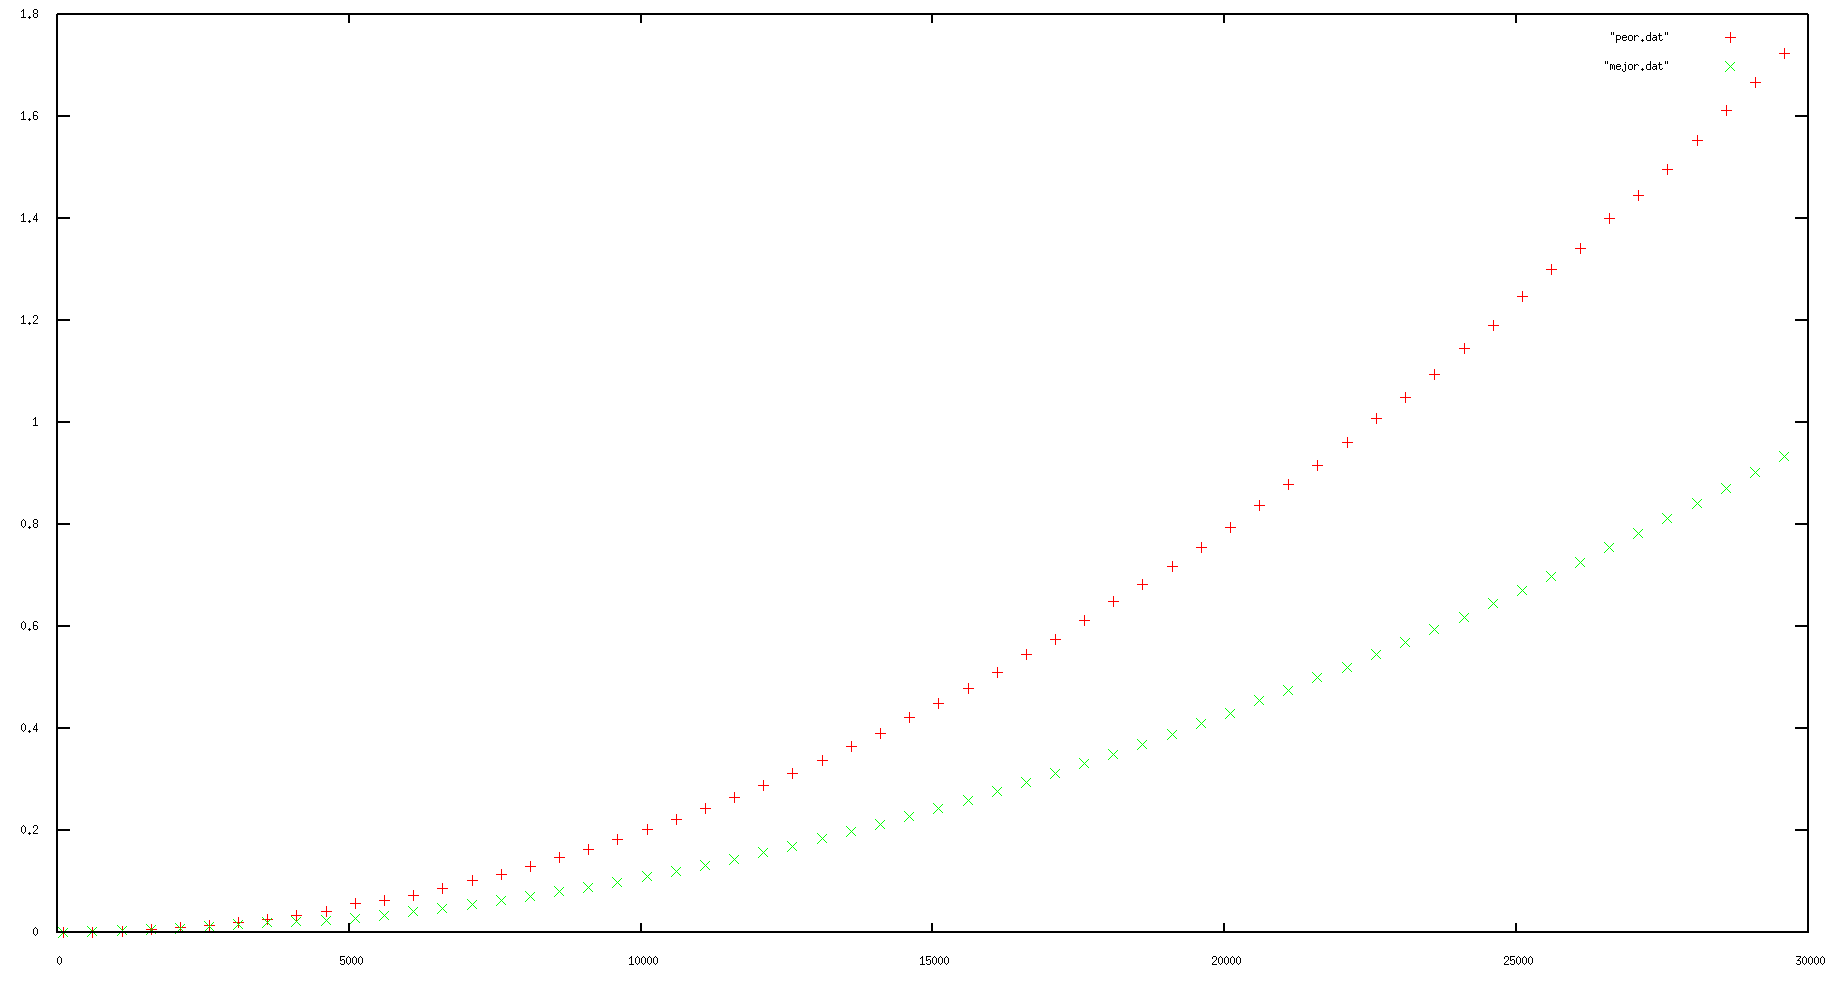
\includegraphics[scale=0.25]{MP.png}

Podemos ver que al inicio ambas tardan el mismo tiempo de ejecución
pero después el caso "peor" empieza a ascender de forma mucho más
rápida en el tiempo de ejecución que la mejor, pues ordenar los datos
que están ordenados al revés es más costoso para burbuja.

\section*{Ejercicio 5}
\label{sec-5}

Con la siguiente implementación del algoritmo burbuja:

\begin{minted}[]{c++}
void ordenar(int *v, int n) { bool cambio=true; //O(1) for (int i=0;
  i<n-1 && cambio; i++) { //O(4) cambio=false; //O(1) for (int j=0;
  j<n-i-1; j++) //O(3) if (v[j]>v[j+1]) { //O(1) cambio=true; //O(1)
  int aux = v[j]; //O(1) v[j] = v[j+1]; //O(1) v[j+1] = aux; //O(1) }
  El if es //O(4) en total } // El bucle for interno es O(n-i)*O(4) }
  //El bucle for externo O(n) }
\end{minted}

En el hipotético caso de que estuviera nuestro vector ordenado,
entonces en el segundo for sólo entraría una vez y cambio se quedaría
en false, saliendo del primer bucle for, por lo que tendríamos $O(n)$
del segundo for por O(1)* del primero, así que la eficiencia teórica
sería $O(n)$ por la notación O.

La empírica total sería, si el vector estuviera ordenado:

\[ O(4)*(O(1)+O(n)) = O(4n + 4) \]

Ahora, podemos dibujar con \emph{gnuplot} la gráfica de la eficiencia empírica:

\includegraphics[scale=0.65]{burbuja2img.png}

Donde podemos observar que nuestra gráfica se ajusta a la previsión que teníamos.

\section*{Ejercicio 6}
\label{sec-6}

Volvemos a compilar nuestro ejercicio de burbuja, usando ahora:

\begin{minted}[]{bash}
g++ -O3 ordenacion.cpp -o ordenacion_optimizado
\end{minted}

Ahora creamos un script para hacer de nuevo las ejecuciones, un script igual que los anteriores pero que ejecute este programa (\emph{ordenacion-optimizado}). 
Seguidamente, creamos nuestra gráfica comparándola con la del ordenación burbuja normal, y el resultado es el siguiente:


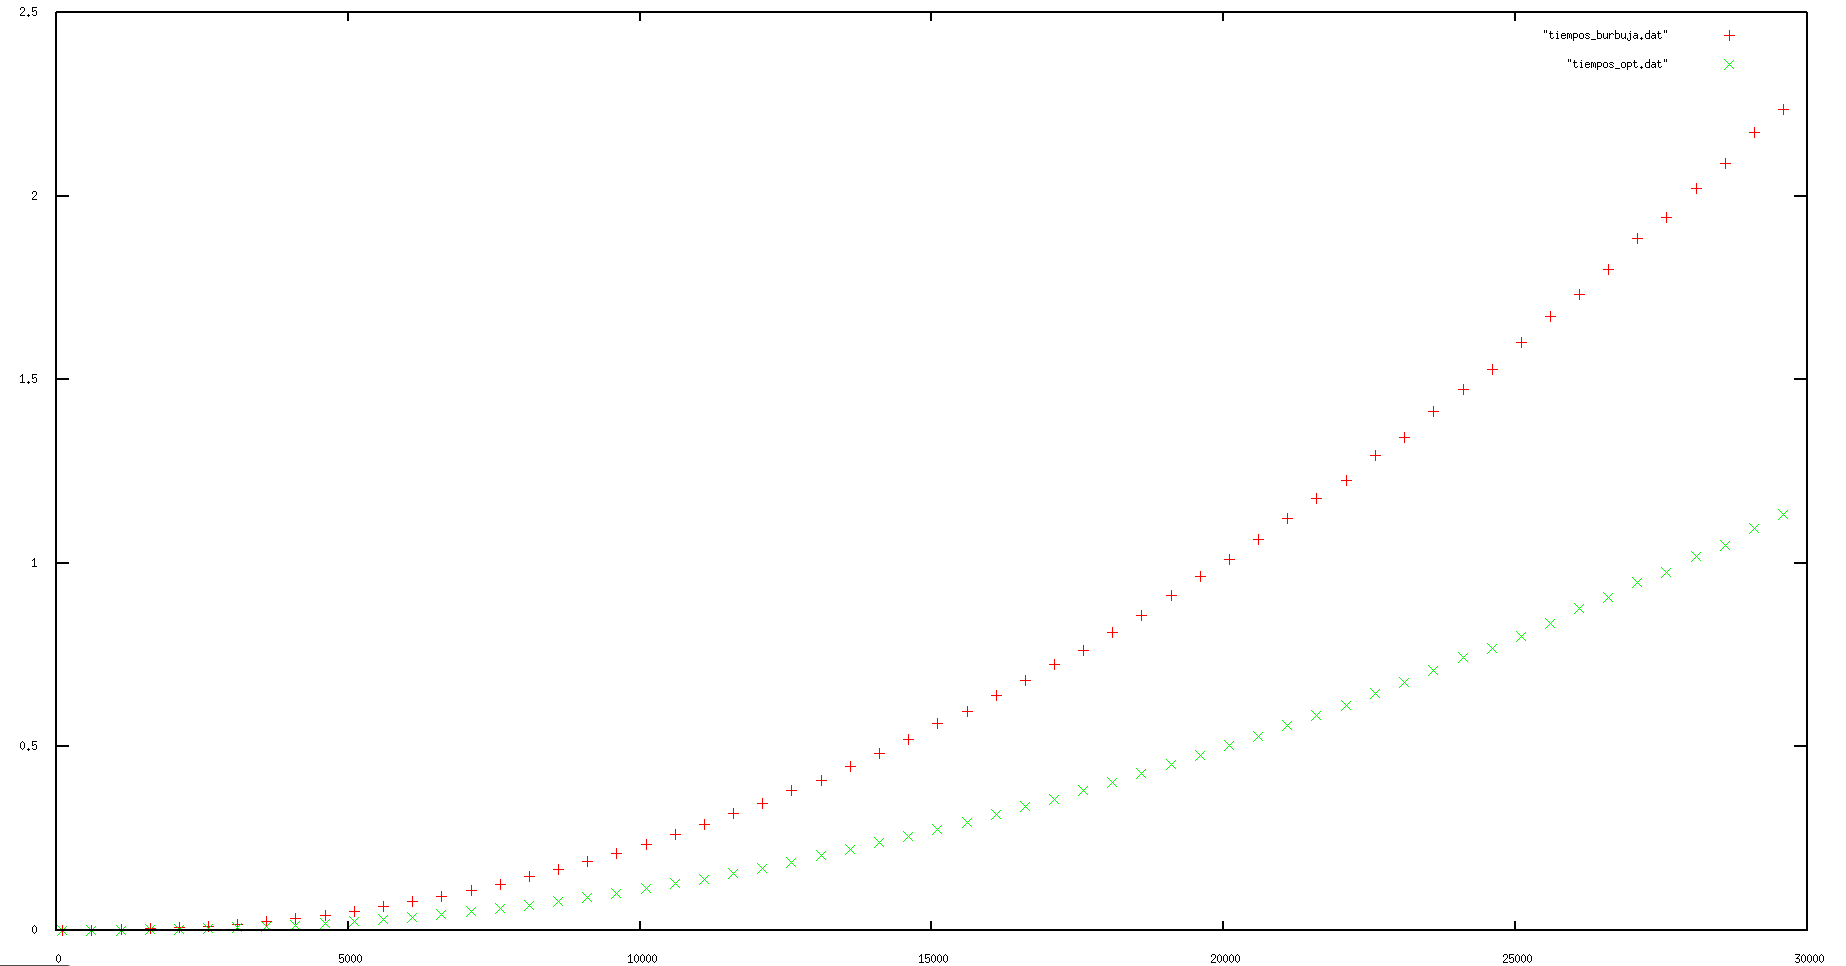
\includegraphics[scale=0.25]{grafica6}

Podemos ver como la compilación optimizada nos ayuda a mejorar mucho la eficiencia de nuestro código, quedando la gráfica de la segunda ejecución optimizado
bastante por debajo de la gráfica de la ejecución que no está optimizada.


\section*{Ejercicio 7}
\label{sec-7}

Vamos a crear primero nuestro programa para las matrices. No vamos a escribirlo entero. Sin embargo, vamos a centrarnos en el algoritmo de multiplicación de
las dos matrices pues sabemos que son 3 bucles for anidados y que por la notación \emph{O} la eficiencia del código será \emph{O} del resultado que de la función
de eficiencia de este algoritmo.
Para ello, suponemos que la primera matriz es de orden \emph{m*n} y la segunda es de orden \emph{n*t}.
Por tanto, el producto sería de orden \emph{m*t}

Analizamos por ello el producto:
\begin{minted}[]{c++}
for (int i = 0; i < filas1; i++){ //O(m)
    for(int j = 0; j < col2; j++){ //O(t)
	producto[i][j] = 0;       //O(1)
	for (int k = 0; k < columnas1; k++)  //O(n)
	     producto[i][j] = producto[i][j] + matrix1[i][k] * matrix2[k][j]; //O(1)
    }
}
\end{minted}

Así, como tenemos 3 bucles \emph{for} anidados, tenemos que aplicar la regla del producto para ver que la eficiencia del programa viene dada por:
\[
O(m)*O(t)*O(n) = O(m*t*n)
\]
Donde, ya sabemos que m son las filas de la 1 matriz, t las columnas d ela segunda matriz, y n las columnas de la primera y las filas de la segunda matriz.

Ahora, si las matrices fuesen cuadradas, serían ambas \emph{n*n} por lo que la eficiencia del código sería $O(n^3)$

Ahora, iremos en busca de la eficiencia empírica ejecutando un script que haga el producto de matrices cuadradas de orden \emph{n*n} variando el n para ver cómo varía
el tiempo de ejecución. Quedando la gráfica de la eficiencia empírica frente a la eficiencia teórica de la siguiente forma:


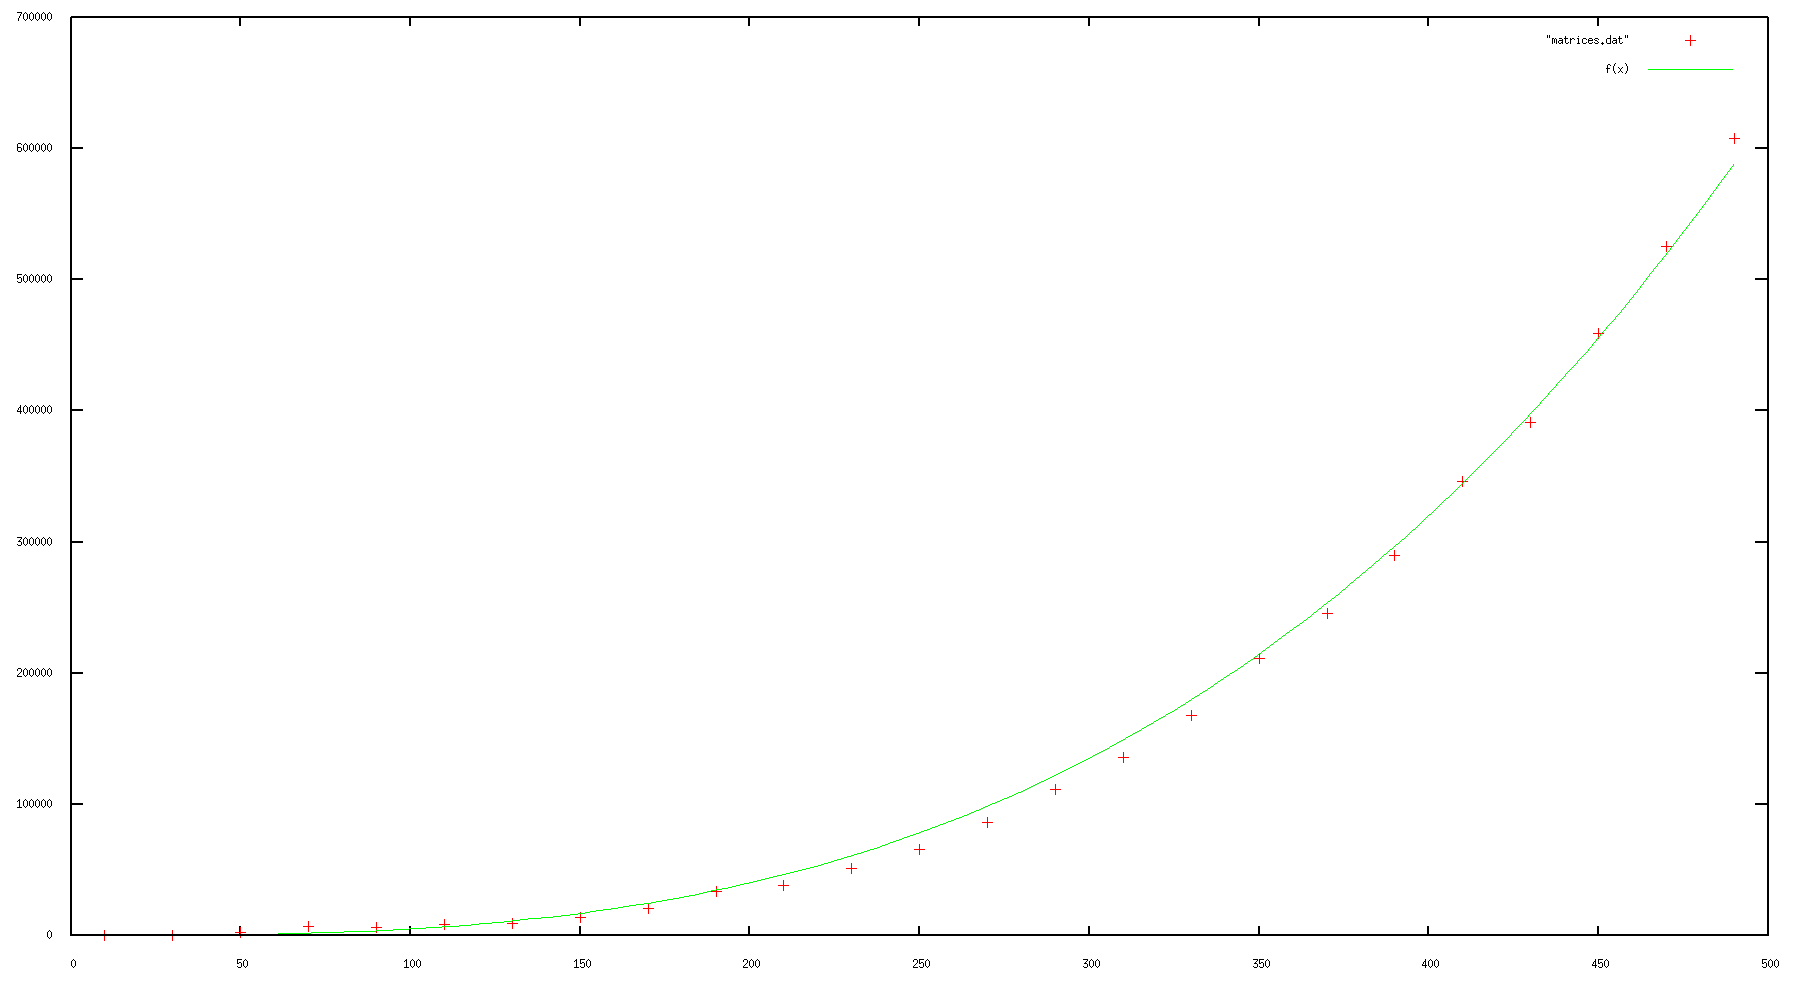
\includegraphics[scale=0.25]{matrices}

\section*{Ejercicio 8}
\label{sec-8}
Vamos a realizar el estudio del algoritmo, primero con el parámetro \verb~UMBRAL_MS~ en 100, que es el por defecto.
El resultado es el siguiente:

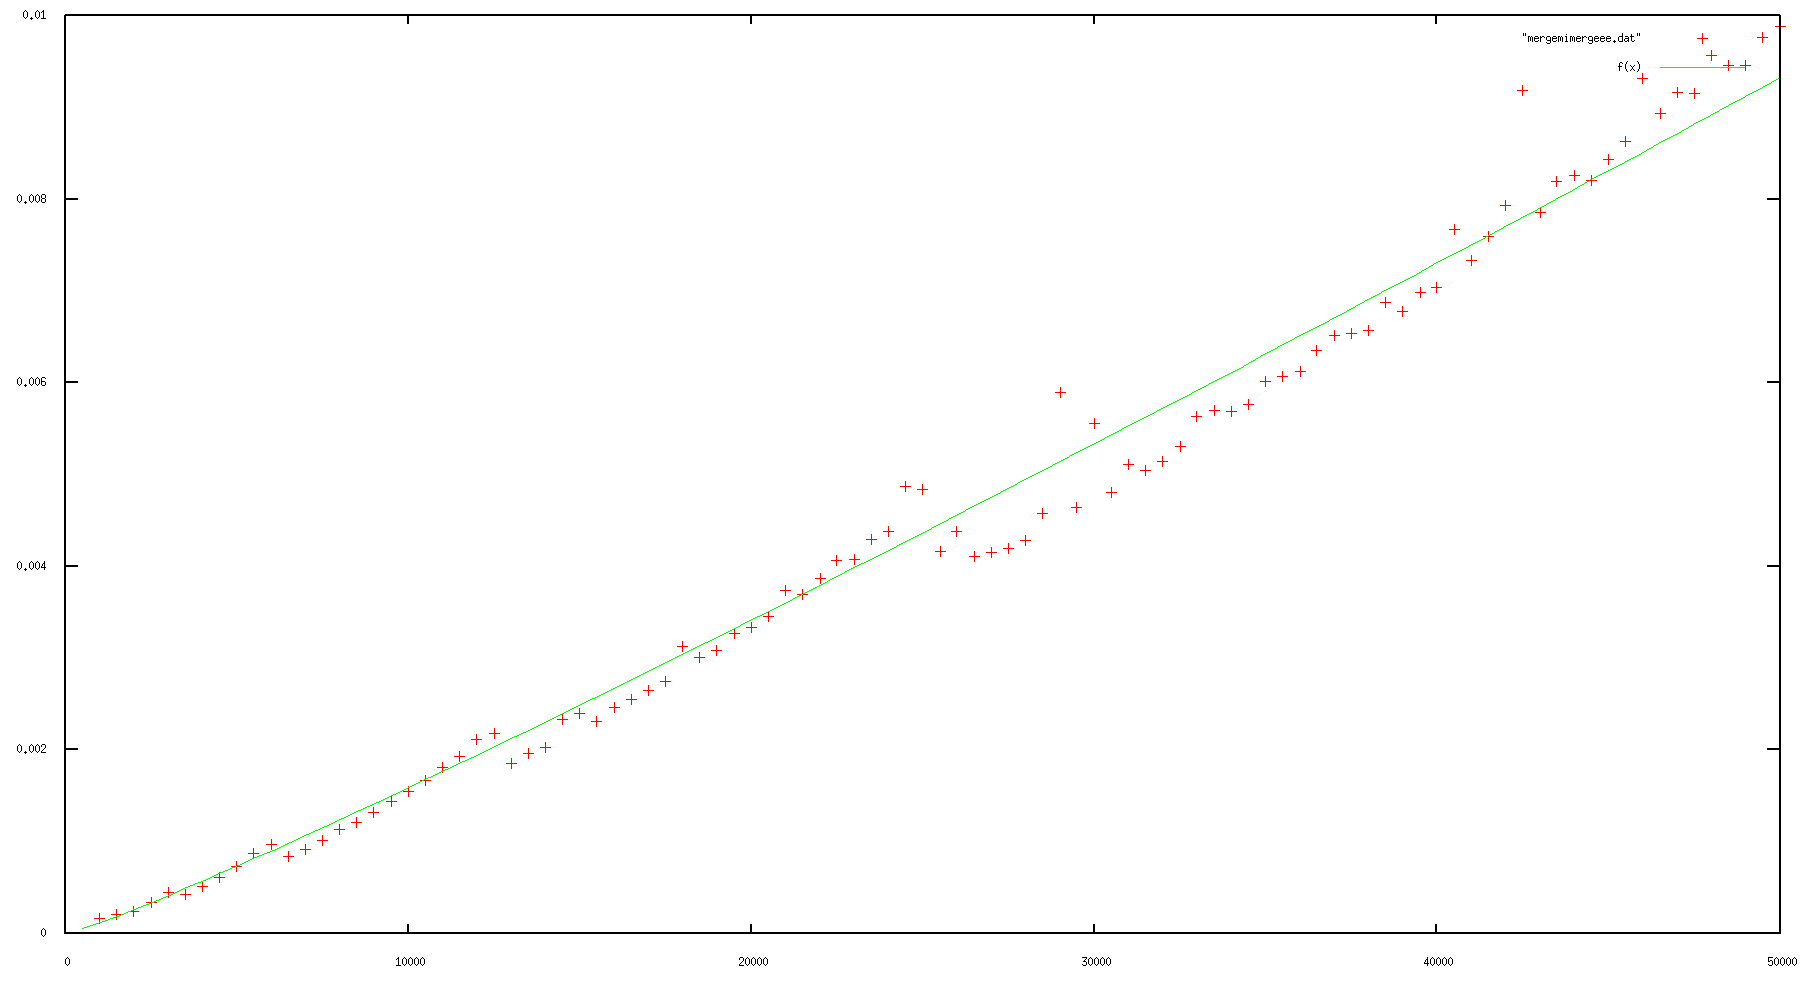
\includegraphics[scale=0.25]{merge1.png}


Ahora, volvemos a ejecutar con \verb~UMBRAL_MS~ en 1000, para ver cómo cambia.

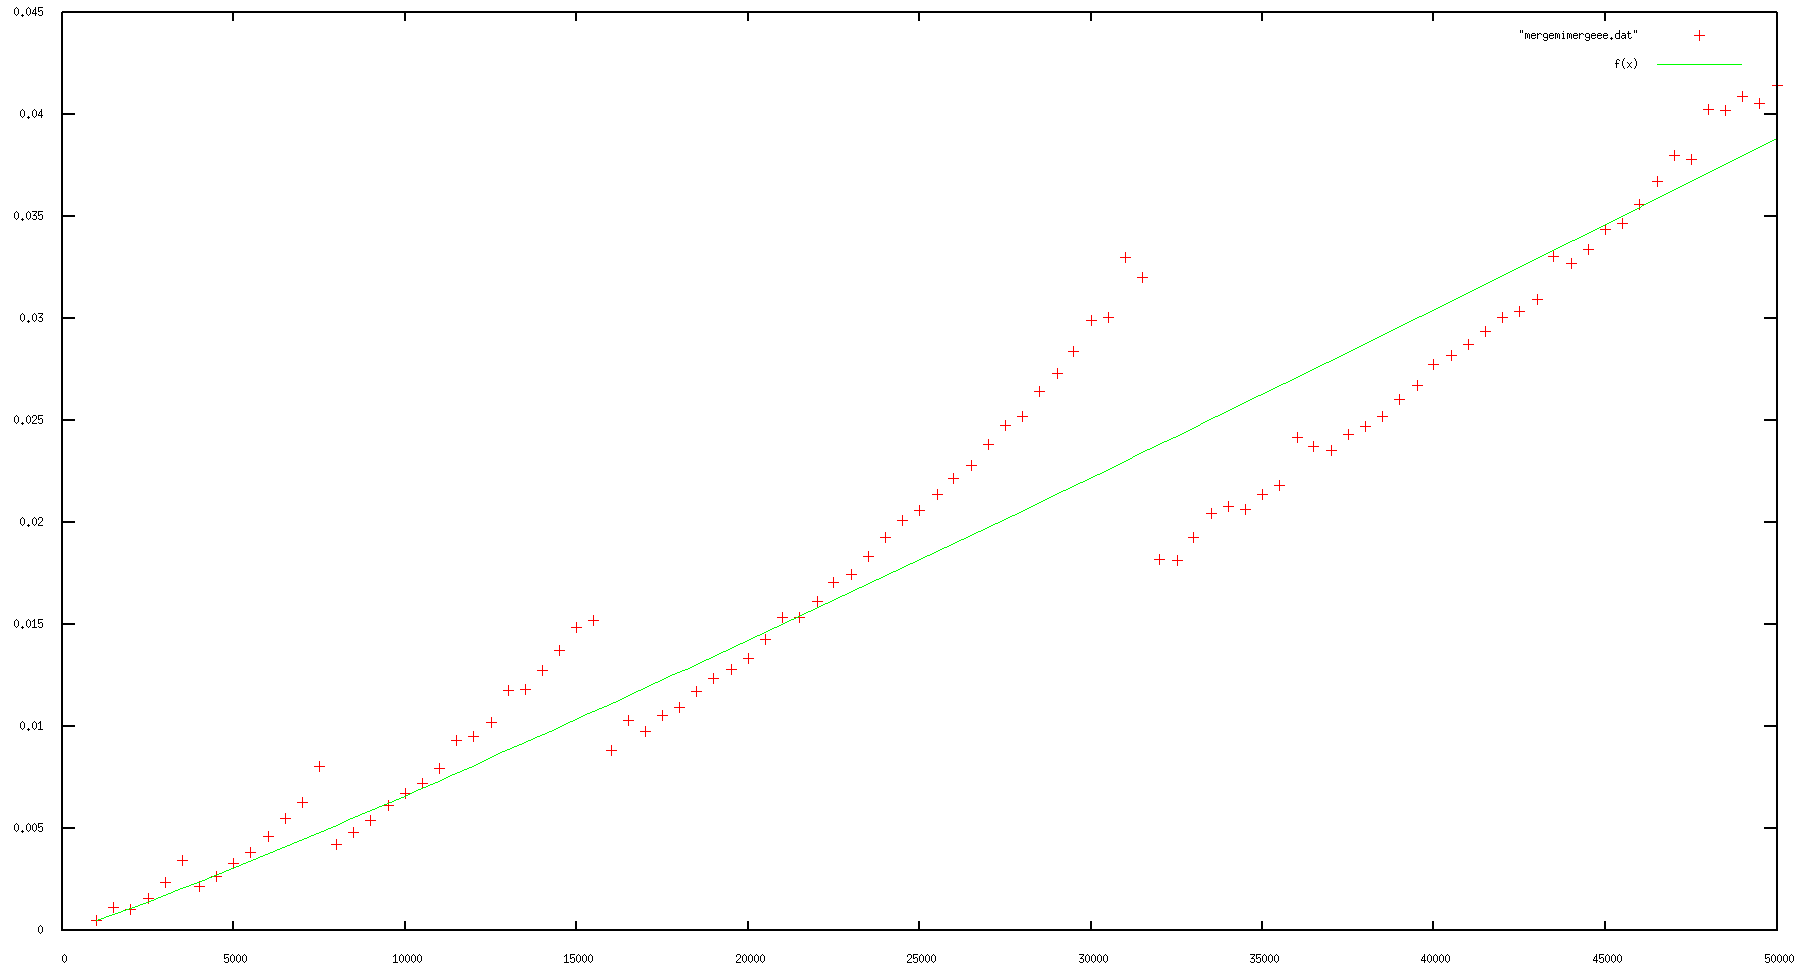
\includegraphics[scale=0.25]{merge2.png}


Por último, ejecutamos el programa con \verb~UMBRAL_MS~ en 10.000, y la gráfica producida es la siguiente.

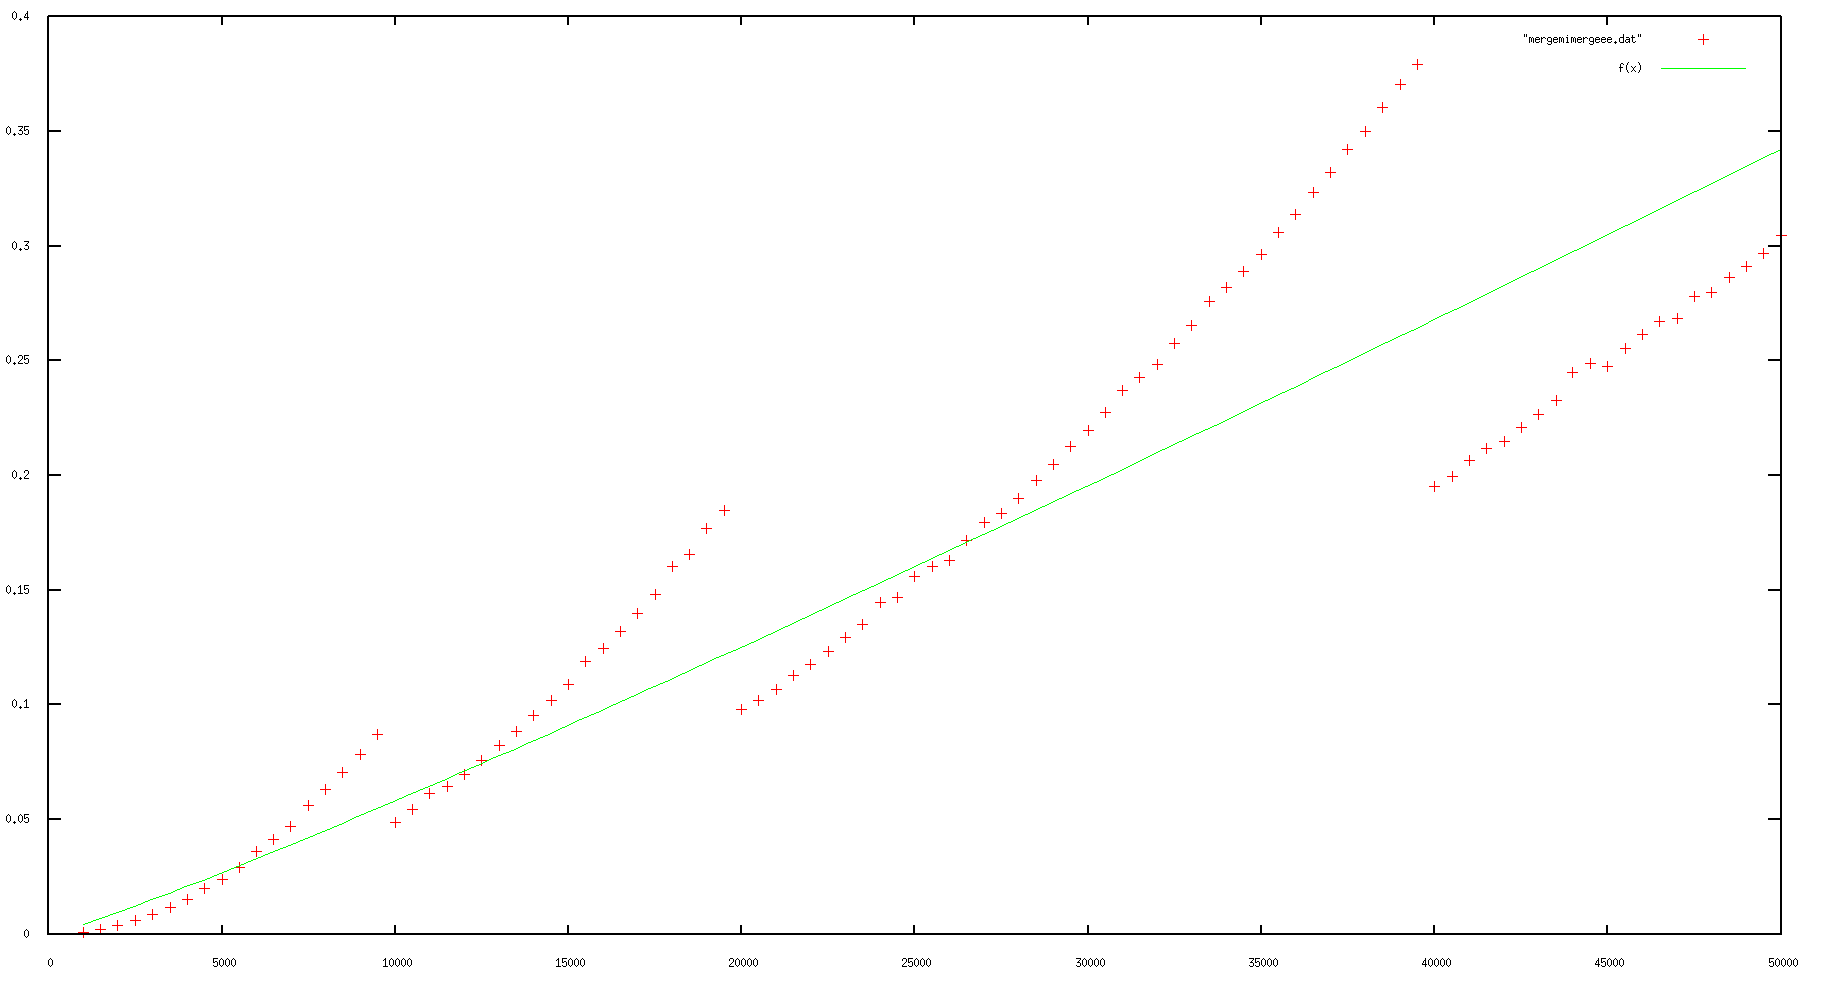
\includegraphics[scale=0.25]{merge3.png}

Al seguir aumentando el \verb~UMBRAL_MS~ el tiempo de ejecución es mucho mayor no por el algoritmo de ordenación
sino porque el programa realiza unas acciones mucho más largas como es copiar el vector varias veces y lo ordena
con mergesort vauna cantidad mucho mayor de veces debido al aumento que hemos realizado del umbral


\section*{Informe de la eficiencia}
\label{sec-9}

\begin{itemize}
\item Hardware utilizado: Hemos utilizado un procesador Intel Core i-7 5700HQ octacore a 2.7 Ghz.Además, el ordenador dispone de 8GB de RAM.
\item Sistema Operativo: GNU Linux. Distribución: Ubuntu 16.04 LTS.
\item Para la compilación hemos usado el compilador de C++ de la GNU
\item El ajuste de las gráficas lo hemos hecho mediante la orden fit de gnuplot.
\end{itemize}
% Emacs 24.5.1 (Org mode 8.2.10)
\end{document}
